\PassOptionsToPackage{unicode=true}{hyperref} % options for packages loaded elsewhere
\PassOptionsToPackage{hyphens}{url}
%
\documentclass[lualatex,b5paper,openany,pandoc,jbase=12Q,magstyle=nomag*]{luakmcbook}

\hypersetup{
            pdftitle={独習KMC vol.~16},
            pdfborder={0 0 0},
            breaklinks=true}

\title{独習KMC vol.~16}
\date{}

% 画像を子ディレクトリから参照したいときは
% \graphicspath{{hoge1/}{hoge2/}} みたいに足していってね
\graphicspath{{./}{recent-kmc/}{utgwkk/}{nana/}}
\usepackage{pdfpages} % \includepdfできるようにする

\begin{document}
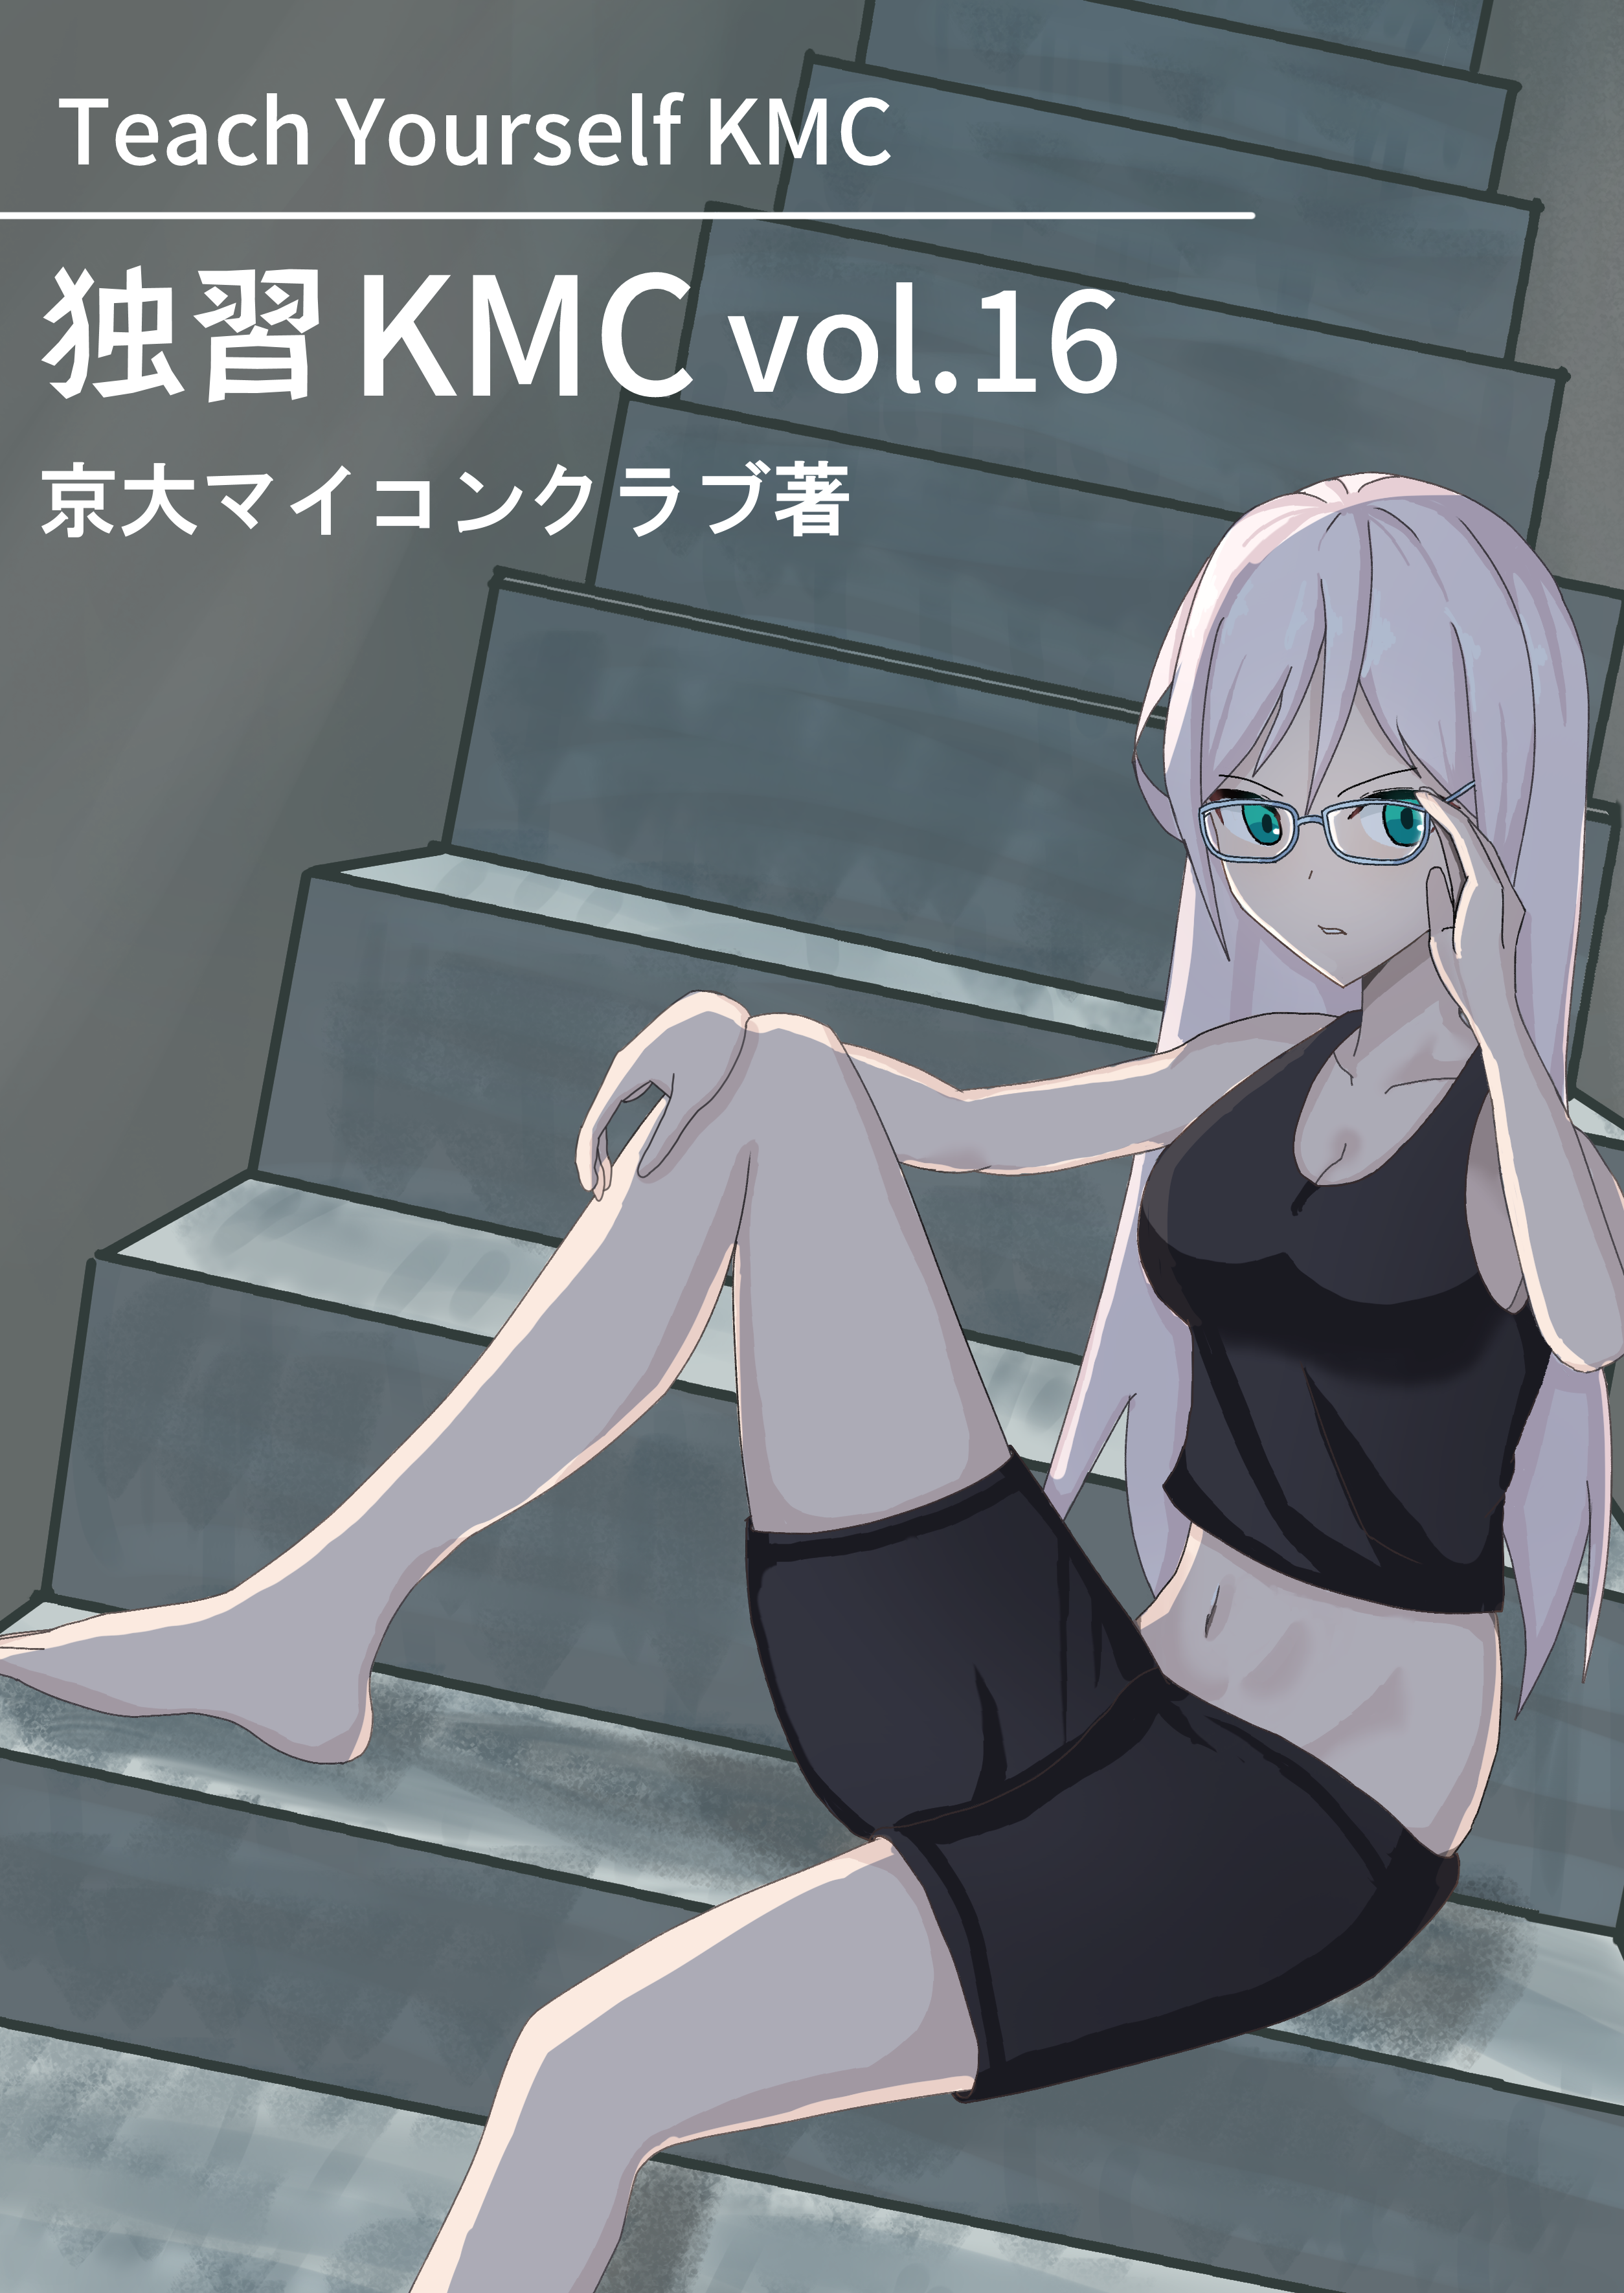
\includepdf{air2_front_5_trim.png}

\maketitle

% 巻頭言
\include{preface}

% 目次生成
\tableofcontents

\part{最近のKMC}
\chapter{最近のKMC --- 役職者より}
恒例の「最近のKMC」コーナーです。
最近のKMCでの活動について、様々な方から寄稿いただきました。

まずは会長と代表からです。

\include*{recent-kmc/kaicho}
\include*{recent-kmc/daihyo}

\chapter{最近のKMC --- 新入生プロジェクト}
次に、毎年新入生向けに開いている「新入生プロジェクト」の担当者からです。

\include*{recent-kmc/kyopro}
\include*{recent-kmc/minge}
\include*{recent-kmc/oekaki}
\include*{recent-kmc/webservice}
\include*{recent-kmc/dtm}

\chapter{最近のKMC --- その他のプロジェクト}
KMCでは、新入生プロジェクト以外にも様々なプロジェクトが動いています。それらの担当者からもコメントをいただきました。

\include*{recent-kmc/clocklock}
\include*{recent-kmc/yasoba}
\include*{recent-kmc/chalk}
\include*{recent-kmc/heavylove}

\part{部員のコラム}
\include{utgwkk/column}
\include{nana/row}
\include{atogaki}

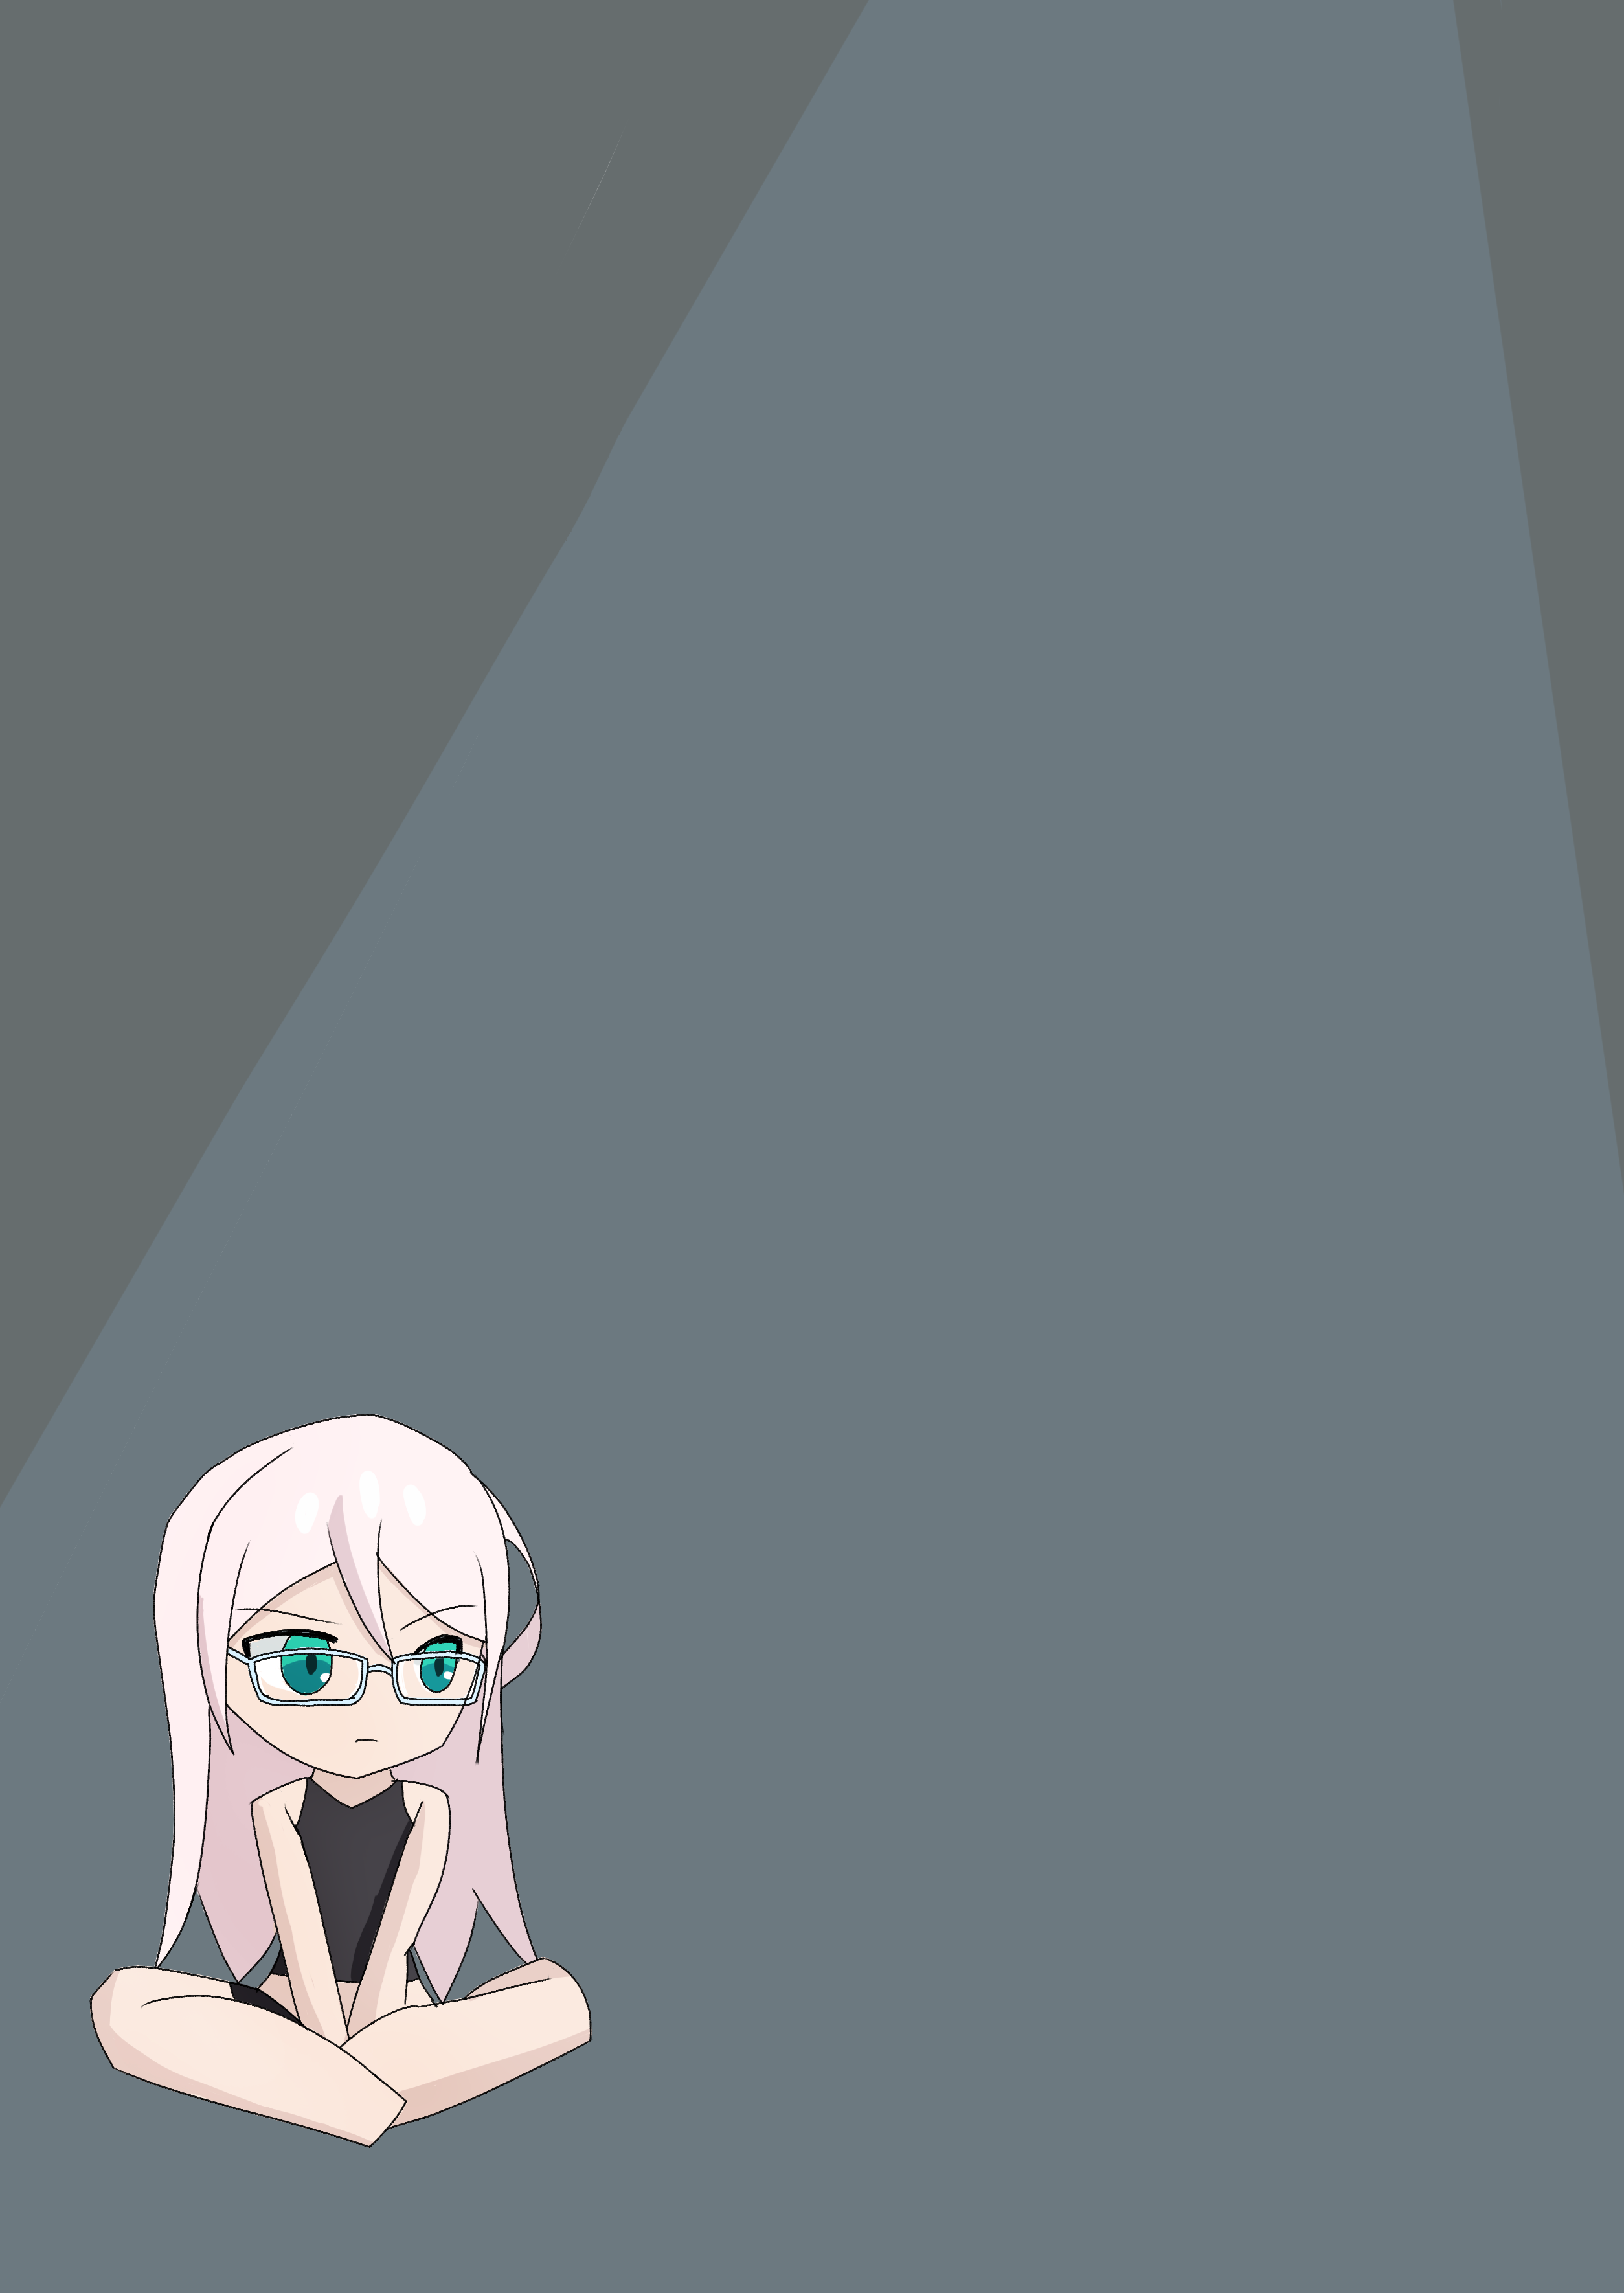
\includepdf{air2_back_trim.png}
\end{document}
